\subsubsection{Workflow der Panoramaerstellung}
\label{sec:Workflow}

Der Workflow der Panoramaerstellung kann in mehrere Teilprozesse untergliedert
werden. Für die Umsetzung dieser einzelnen Teilschritte wird hierbei spezielles
Hard- und Softwareequipment benötigt. Im Folgenden sollen die einzelnen
Teilschritte der Panoramaerstellung in chronologischer Reihenfolge erläutert
werden. Im Zuge dessen soll auch auf das benötigte Equipment eingegangen
werden.

\paragraph{Aufnahme der Einzelfotos} \hfill \\

Die Panoramaerstellung beginnt mit der Aufnahme mehrerer Einzelfotos. Aus diesen
Einzelfotos wird nachfolgend dann das komplette Panoramafoto zusammengefügt.
Dieses muss, wie zuvor erläutert, der Rektangularprojektion entsprechen. Die
Summe der Einzelfotos muss also eine horizontale Ansicht von 360 Grad und eine
vertikale Ansicht von 180 Grad abbilden. Die Anzahl der Einzelfotos ist somit
von dem Bildwinkel abhängig, der auf einem einzelnen Foto dargestellt werden
kann. Dieser Bildwinkel wird in der Fotografie durch die Brennweite des
Objektives festgelegt. Je geringer die Brennweite eines Objektives ist, desto
größer ist der Bildwinkel, der mit diesem Objektiv eingefangen werden kann und
desto weniger Einzelfotos werden für die Erstellung eines Panoramafotos
benötigt. Durch spezielle Objektivkonstruktionen wie zum Beispiel einem
Fisheye-Obektiv ist es möglich einen besonders großen Bildwinkel aufzunehmen.
Ein solches Objektiv und eine zum dem Objektiv kompatible Kamera wird auch für die Aufnahme der
Panoramafotos im Projekt verwendet. Das Objektiv ermöglicht es in 16 Fotos alle
Ansichten Aufzunehmen, die zur Darstellung einer Rektangularprojektion benötigt
werden. In 15 dieser Einzelfotos ist hierbei die horizontale Rundumansicht
dargestellt. Das sechzehnte Foto bildet den Zenit\footnote{Der Zenit ist der
Punkt über dem Beobachter/der Kamera} im Panoramafoto ab. Der
Nadir\footnote{Der Nadir ist der dem Zent gegenüber gelegene Punkt unter dem
Beobachter/der Kamera} wird in den Panoramafotos nicht abgebildet, da sich hier
das Stativ befindet.

Zur Unterstützung bei der Aufnahme hat sich die Projektgruppe weiterhin
entschieden ein speziell für die Panoramafotografie ausgelegtes Stativ zu
verwenden. Eine Aufnahme ohne dieses Stativ wäre zwar denkbar, würde die
Qualität der Panoramafotos jedoch stark beeinträchtigen. Das Panoramastativ
besteht aus folgenden Komponenten:

\begin{description}
\item[Stativ] Das eigentliche Stativ dient dazu, die Kamera im Raum an einer
festen Position zu fixieren. Hierdurch ist sichergestellt, dass alle
Einzelfotos von der selben Position aus aufgenommen werden.
\item[Nivelliervorrichtung] Die Nivelliervorrichtung dient dazu, den Kopf des
Statives horitontal auszurichten. Auf diese Weise wird ein wellenförmiger
Horizont in dem zusammengefügten Panoramafoto vermieden.
\item[Rotator] Der Rotator ermöglicht es, den Kopf des Stativs um die vertikale
Achse zu drehen. Weiterhin kann eine Gradzahl festgelegt werden, nachdem der
Machanismus bei einer Drehnung einrastet. Auf diese Weise wird eine gleichmäßige
Drehung bei der Aufnahme der Panoramafotos ermöglicht.
\item[Nodalpunktadapter] Der Nodalpunktadapter ermöglicht es, die Kamera auf
dem Stativ so zu positionieren, dass die Eintrittspupille des Stativs auf Höhe
der vertikalen Drehachse des Stativs liegt. Hierdurch können
Parallaxenfehler\footnote{Der Parallaxenfehler beschreibt eine scheinbare
Verschiebung zweier hintereinandergelegener Gegenstände, wenn sich der
Ausgangspunkt der Betrachtung ändert} bei der Aufnahme vermieden werden
\end{description}

Das komplette Equipment, welches zur Aufnahme der Panoramafotos verwendet wurde,
ist in \abbildung{Equipment} dargestellt.

\begin{figure}[htb]
\centering
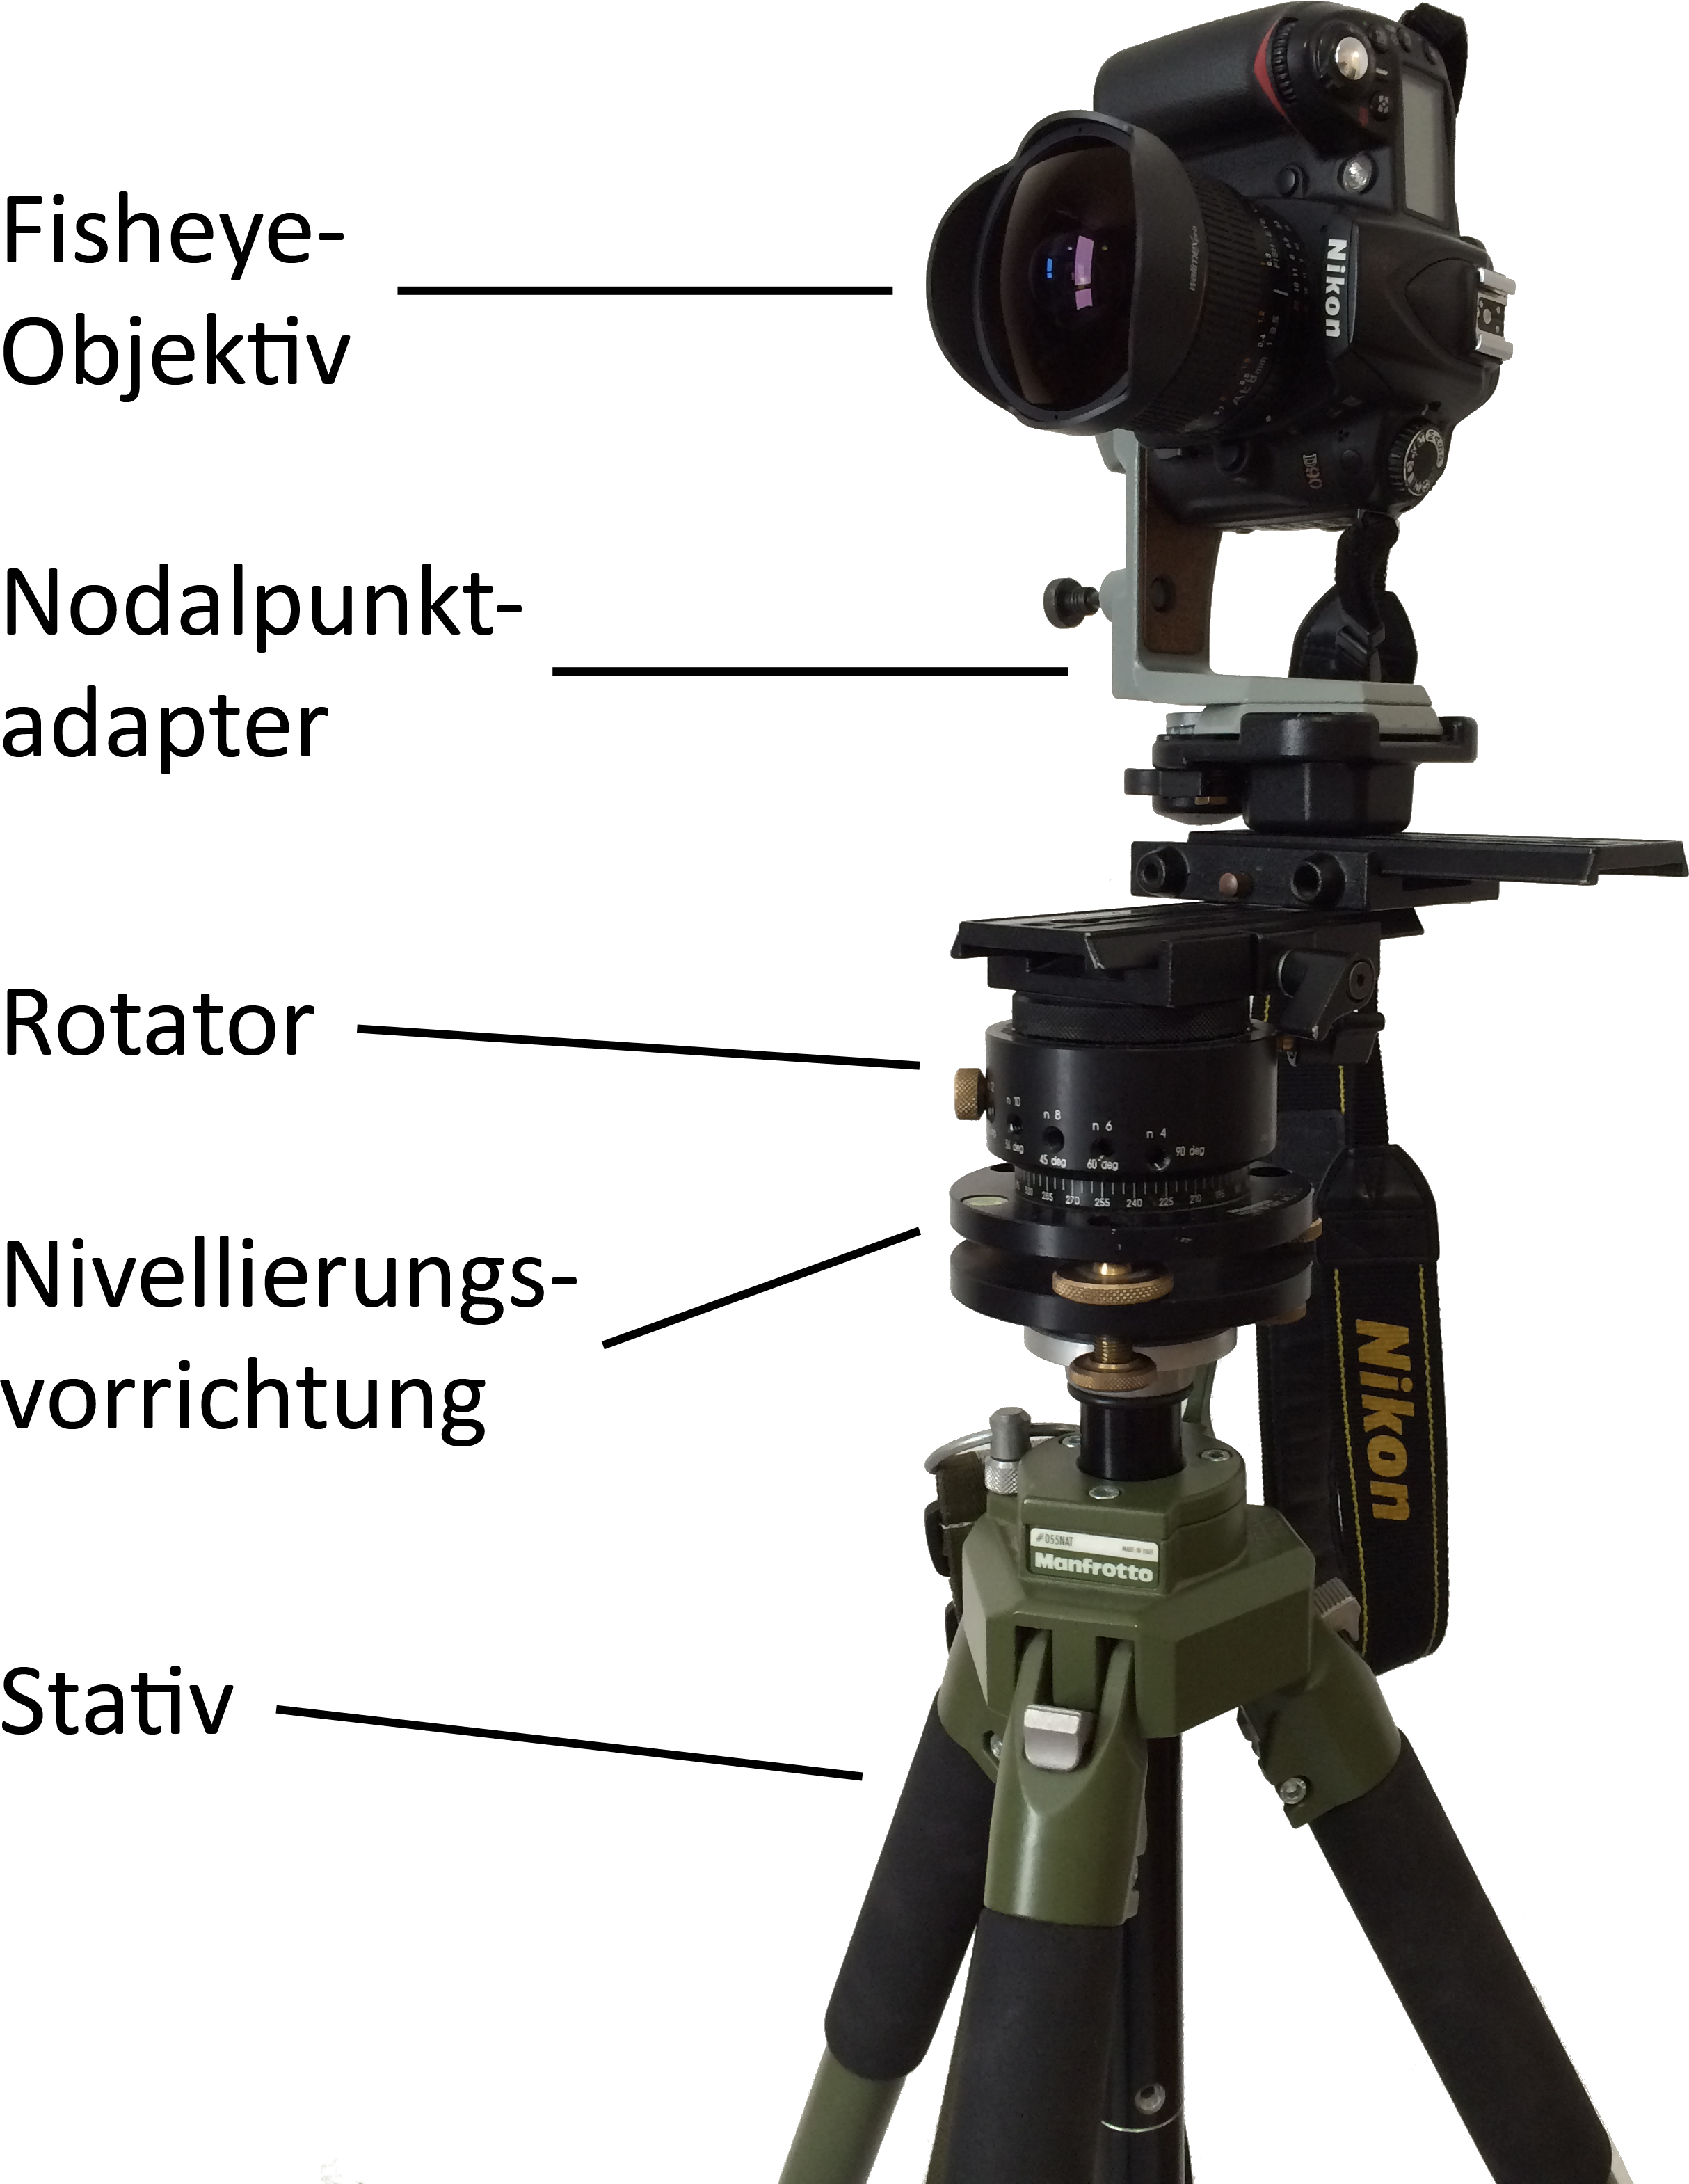
\includegraphics[width=0.5\textwidth]{Equipment.png}
\caption[Equipment zur Aufnahme der Einzelfotos]{Equipment zur Aufnahme der Einzelfotos\protect\footnotemark}
\label{fig:Equipment}
\end{figure}
\footnotetext{Eigene Darstellung}

\paragraph{Stitching und Rendering} \hfill \\

Nachdem die Einzelfotos aufgenommen wurden müssen diese zu einem Panoramafoto
zusammengefügt werden. Dieser Prozess wird als Stitching bezeichnet. Das
Stitching erfolgt im Projekt mit der Software Kolor Autopano Giga 3.0. Die
Software ist in der Lage, die Einzelfotos automatisiert zusammenzufügen.
Gegebenenfall muss das hieraus resultierende Panoramafoto nach dem
automatisierten Zusammenfügen noch manuell ausgerichtet werden. Aufgrund
dieser manuellen Ausrichtung ist es nicht möglich, den hier beschriebenen
Prozess vollständig zu automatisieren. In einem letzen Schritt wird das
zusammengefügte Panoramafoto dann in das JPEG-Format konvertiert. Dieser Schritt
wird als Rendering bezeichnet. Das Ergebnis dieses Prozesses ist in
\abbildung{Zusammengefuegt} dargestellt.

\begin{figure}[htb]
\centering
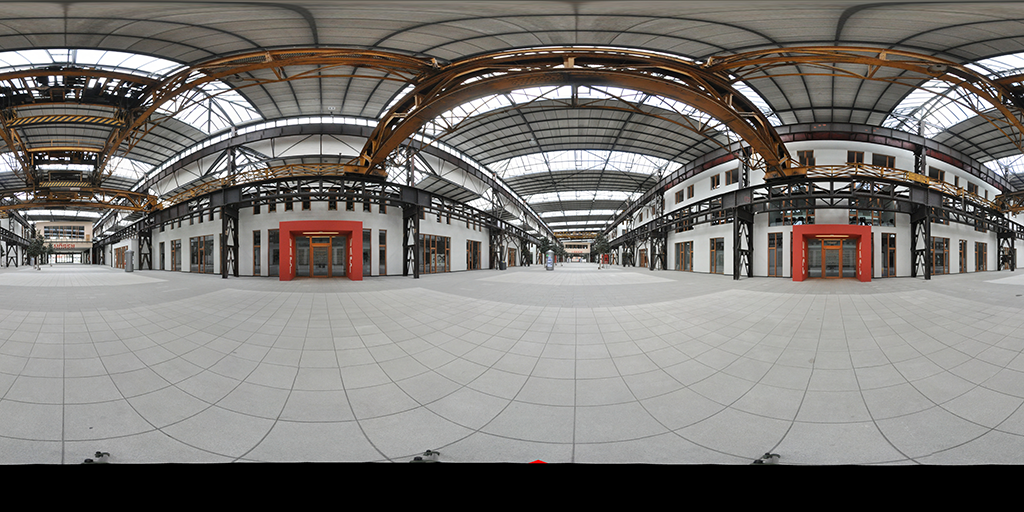
\includegraphics[width=0.8\textwidth]{Zusammengefuegt.png}
\caption[Panoramafoto nach Stitching und Rendering]{Panoramafoto nach Stitching
und Rendering\protect\footnotemark}
\label{fig:Zusammengefuegt}
\end{figure}
\footnotetext{Eigene Darstellung}

\paragraph{Überarbeitung und Optimierung der Panoramafotos} \hfill \\

Da es bei der Aufnahme der Einzelfotos nicht möglich war den Nadir abzubilden,
fehlen diese Informationen folglich auch in dem zusammengefügten
Pa\-no\-ra\-ma\-fo\-to. In \abbildung{Zusammengefuegt} ist der Bereich, in dem
die Bildinformationen fehlen, durch eine schwarze Fläche markiert. Im Zuge
einer Überarbeitung der Panoramafotos soll dieser schwarze Bereich mit einem
Label überdeckt werden, auf dem das Logo des Projektes dargestellt ist. Das
Label muss dabei so verzerrt werden, dass es nach der bereits beschriebenden
Projezierung durch die Google Street View API entzerrt dargestellt ist.

Neben der Überarbeitung der Panoramafotos werden diese weiterhin für die
Darstellung im Internet optimiert. Hierbei wird die Größe des Panoramafotos auf
die Pixelmaße 4096x2048 reduziert und die JPEG-Datei komprimiert abgesspeichert.

Die Bearbeitung der Panoramafotos erfolgt mit der Software Adobe Photoshop CS5.
Durch die Stapelverarbeitungsfunktion des Programms können alle hier
beschriebenen Teilschritte automatisiert durchgeführt werden. Das Ergebnis
dieses Prozesses ist in \abbildung{Ueberarbeitet} dargestellt.

\begin{figure}[htb]
\centering
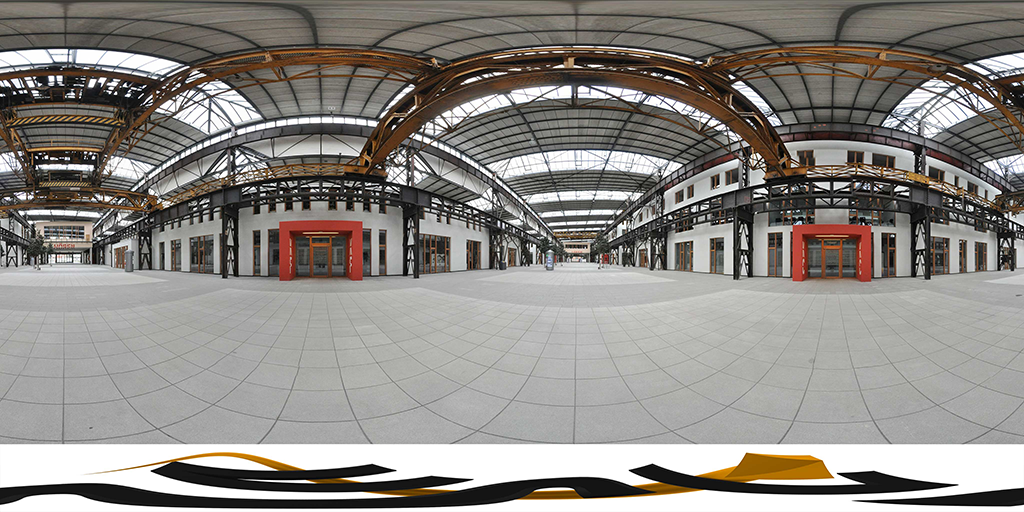
\includegraphics[width=0.8\textwidth]{Ueberarbeitet.png}
\caption[Panoramafoto nach Überarbeitung und Optimierung]{Panoramafoto nach
Überarbeitung und Optimierung\protect\footnotemark}
\label{fig:Ueberarbeitet}
\end{figure}
\footnotetext{Eigene Darstellung}

\paragraph{Aufteilung des Panoramafotos in Kacheln} \hfill \\

Das Blickfeld des Benutzers in der Anwendung nimmt immer nur einen Teil der
Rundumansicht ein. Somit kann auch immer nur ein Teil des Panoramafotos
dargestellt werden. Es ist daher nicht sinnvoll das komplette Panoramafoto in
der Anwendung zu laden, bevor es dem Benutzer präsentiert wird.
Aus diesem Grund wird das Panoramafoto in einem letzten Bearbeitungsschritt in
mehrere Kacheln aufgeteilt. Ziel dieser Aufteilung ist eine Steigerung der
Performanz und eine Reduzierung der Ladezeiten für die Panoramafotos in der
Anwendung. Es muss immer nur der Teil der Kacheln geladen werden, der dem
Benutzer aktuell präsentiert wird. Wenn sich das Blickfeld des Benutzers ändert
können einzelne Kacheln schnell nachgeladen werden.

Die Aufteilung der Panoramafotos im Projekt erfolgt, wie auch die Überarbeitung
der Fotos, mit der Software Adobe Photoshop CS5. Auch hier kann die
Stapelverarbeitungsfunktion genutzt werden, um die Aufteilung der Panoramafotos
zu automatisieren.
